\documentclass[xcolor={dvipsnames}]{beamer}
%\usepackage[utf8]{inputenc}
\usetheme{Madrid}
%\usetheme{Malmoe}
\usecolortheme{beaver}
%\usecolortheme{rose}

%-------------------------------------------------------------------------------
%          -Packages nécessaires pour écrire en Français et en UTF8-
%-------------------------------------------------------------------------------
\usepackage[utf8]{inputenc}
\usepackage[frenchb]{babel}
\usepackage[T1]{fontenc}
\usepackage{lmodern}
\usepackage{textcomp}

%-------------------------------------------------------------------------------

%-------------------------------------------------------------------------------
%                          -Outils de mise en forme-
%-------------------------------------------------------------------------------
\usepackage{hyperref}
\hypersetup{pdfstartview=XYZ}
\usepackage{enumerate}
\usepackage{graphicx}
%\usepackage{multicol}
%\usepackage{tabularx}

%\usepackage{anysize} %%pour pouvoir mettre les marges qu'on veut
%\marginsize{2.5cm}{2.5cm}{2.5cm}{2.5cm}

\usepackage{indentfirst} %%pour que les premier paragraphes soient aussi indentés
\usepackage{verbatim}
%\usepackage[table]{xcolor}  
%\usepackage{multirow}
\usepackage{ulem}
%-------------------------------------------------------------------------------


%-------------------------------------------------------------------------------
%                  -Nécessaires pour écrire des mathématiques-
%-------------------------------------------------------------------------------
\usepackage{amsfonts}
\usepackage{amssymb}
\usepackage{amsmath}
\usepackage{amsthm}
\usepackage{tikz}
\usepackage{xlop}
\usepackage[output-decimal-marker={,}]{siunitx}
%-------------------------------------------------------------------------------


%-------------------------------------------------------------------------------
%                    - Mise en forme 
%-------------------------------------------------------------------------------

\newcommand{\bu}[1]{\underline{\textbf{#1}}}


\usepackage{ifthen}


\newcommand{\ifTrue}[2]{\ifthenelse{\equal{#1}{true}}{#2}{$\qquad \qquad$}}

\newcommand{\kword}[1]{\textcolor{red}{\underline{#1}}}


%-------------------------------------------------------------------------------



%-------------------------------------------------------------------------------
%                    - Racourcis d'écriture -
%-------------------------------------------------------------------------------

% Angles orientés (couples de vecteurs)
\newcommand{\aopp}[2]{(\vec{#1}, \vec{#2})} %Les deuc vecteurs sont positifs
\newcommand{\aopn}[2]{(\vec{#1}, -\vec{#2})} %Le second vecteur est négatif
\newcommand{\aonp}[2]{(-\vec{#1}, \vec{#2})} %Le premier vecteur est négatif
\newcommand{\aonn}[2]{(-\vec{#1}, -\vec{#2})} %Les deux vecteurs sont négatifs

%Ensembles mathématiques
\newcommand{\naturels}{\mathbb{N}} %Nombres naturels
\newcommand{\relatifs}{\mathbb{Z}} %Nombres relatifs
\newcommand{\rationnels}{\mathbb{Q}} %Nombres rationnels
\newcommand{\reels}{\mathbb{R}} %Nombres réels
\newcommand{\complexes}{\mathbb{C}} %Nombres complexes


%Intégration des parenthèses aux cosinus
\newcommand{\cosP}[1]{\cos\left(#1\right)}
\newcommand{\sinP}[1]{\sin\left(#1\right)}

%Fractions
\newcommand{\myfrac}[2]{{\LARGE $\frac{#1}{#2}$}}

%Vocabulaire courrant
\newcommand{\cad}{c'est-à-dire}

%Droites
\newcommand{\dte}[1]{droite $(#1)$}
\newcommand{\fig}[1]{figure $#1$}
\newcommand{\sym}{symétrique}
\newcommand{\syms}{symétriques}
\newcommand{\asym}{axe de symétrie}
\newcommand{\asyms}{axes de symétrie}
\newcommand{\seg}[1]{$[#1]$}
\newcommand{\monAngle}[1]{$\widehat{#1}$}
\newcommand{\bissec}{bissectrice}
\newcommand{\mediat}{médiatrice}
\newcommand{\ddte}[1]{$[#1)$}

%Figures
\newcommand{\para}{parallélogramme}
\newcommand{\paras}{parallélogrammes}
\newcommand{\myquad}{quadrilatère}
\newcommand{\myquads}{quadrilatères}
\newcommand{\co}{côtés opposés}
\newcommand{\diag}{diagonale}
\newcommand{\diags}{diagonales}
\newcommand{\supp}{supplémentaires}
\newcommand{\car}{carré}
\newcommand{\cars}{carrés}
\newcommand{\rect}{rectangle}
\newcommand{\rects}{rectangles}
\newcommand{\los}{losange}
\newcommand{\loss}{losanges}


%----------------------------------------------------


\usepackage{../../../../pas-math}
\usepackage{../../../../moncours_beamer}

\usepackage{amssymb,amsmath}


\newcommand{\myitem}{\item[\textbullet]}

\graphicspath{{../img/}}

\title{Chapitre 1 : Nombre entiers et décimaux}
%\author{O. FINOT}\institute{Collège S$^t$ Bernard}

%
\AtBeginSection[]
{
	\begin{frame}
		\frametitle{}
		\tableofcontents[currentsection, hideallsubsections]
	\end{frame} 

}
%
%
%\AtBeginSubsection[]
%{
%	\begin{frame}
%		\frametitle{Sommaire}
%		\tableofcontents[currentsection, currentsubsection]
%	\end{frame} 
%}

\begin{document}



\begin{frame}
  \titlepage 
\end{frame}


	
\begin{frame}
	\begin{block}{Objectifs}
		\begin{itemize}
			\item Savoir placer les chiffres d'un nombre jusqu'au milliard et à la 4$^{ème}$ décimale;
			\item Savoir multiplier et diviser un nombre par 10, 100 et 1000;
			\item Connaître les fractions décimales.		
		\end{itemize}
	\end{block}
\end{frame}


\section{\'Ecrire un nombre}




\begin{frame}{}

	\begin{block}{Activité 1 Différentes écritures d'un nombre}
		\begin{enumerate}\pause
			\item 
			\begin{itemize}
				\item 17 et 42 sont des nombres à 2 chiffres;\pause
				\item 128 et 512 sont des nombres à 3 chiffres;\pause
				\item \num{2048} et \num{4096} sont des nombres à 4 chiffres;\pause
				\item \num{16384} et \num{65536} sont des nombres à 5 chiffres.\pause
			\end{itemize}
			
			%\item \'Ecrire les nombres suivants en toutes lettres : \num{32}, \num{128} et \num{1024}. 
			\item Le nombre 25146041337 s'écrit \num{25146041337}.\pause
			\item 
			\begin{itemize}
				\item 3,4 milliers s'écrit \num{3400};\pause
				\item 144,8 millions s'écrit \num{144800000};\pause
				\item 163 milliards s'écrit \num{163000000000}.\pause
			\end{itemize}
			
			\item .
			\begin{itemize}
				\item Cinq-cent-un-millions-six-cent-vingt-deux-mille-sept-cent-trente-et-un s'écrit \num{501622731};\pause
				\item Cinq-cent-millions s'écrit \num{500000000}.\pause
			\end{itemize}
			
		\end{enumerate}
	\end{block}
\end{frame}



\begin{frame}
	\begin{alertblock}{Définitions}
		\begin{itemize}\pause
			\item Il existe 10 \kword{chiffres} : 0, 1, 2, 3, 4, 5, 6, 7, 8 et 9.\pause
			
			\item On utilise les chiffres pour écrire des \kword{nombres}.\pause	
		
		\end{itemize}
	\end{alertblock}

	\begin{exampleblock}{Exemples}
		\begin{itemize}
			\item Avec les chiffres 2 et 4 on peut écrire les nombres \pause 24 et 42.\pause
			\item Le nombre \num{4096} s'écrit avec les chiffres 4, 0, 9 et 6.
			
		\end{itemize}
	\end{exampleblock}

	
\end{frame}



\begin{frame}
	\begin{alertblock}{Définitions}
		\begin{itemize}\pause
			\item Pour mieux lire un grand nombre, on regroupe ses chiffres en classes par groupe de 3.\pause
			
			\item Un \kword{nombre décimal} possède une \kword{partie entière} (avant la virgule) et une \kword{partie décimale} (après la virgule).\pause
			
			\item Un nombre décimal où la partie décimale ne contient que des zéros est un \kword{nombre entier}. Dans ce cas la partie décimale n'apparait pas.	
			
		\end{itemize}
	\end{alertblock}	
	
\end{frame}




\begin{frame}
	
	\begin{center}
		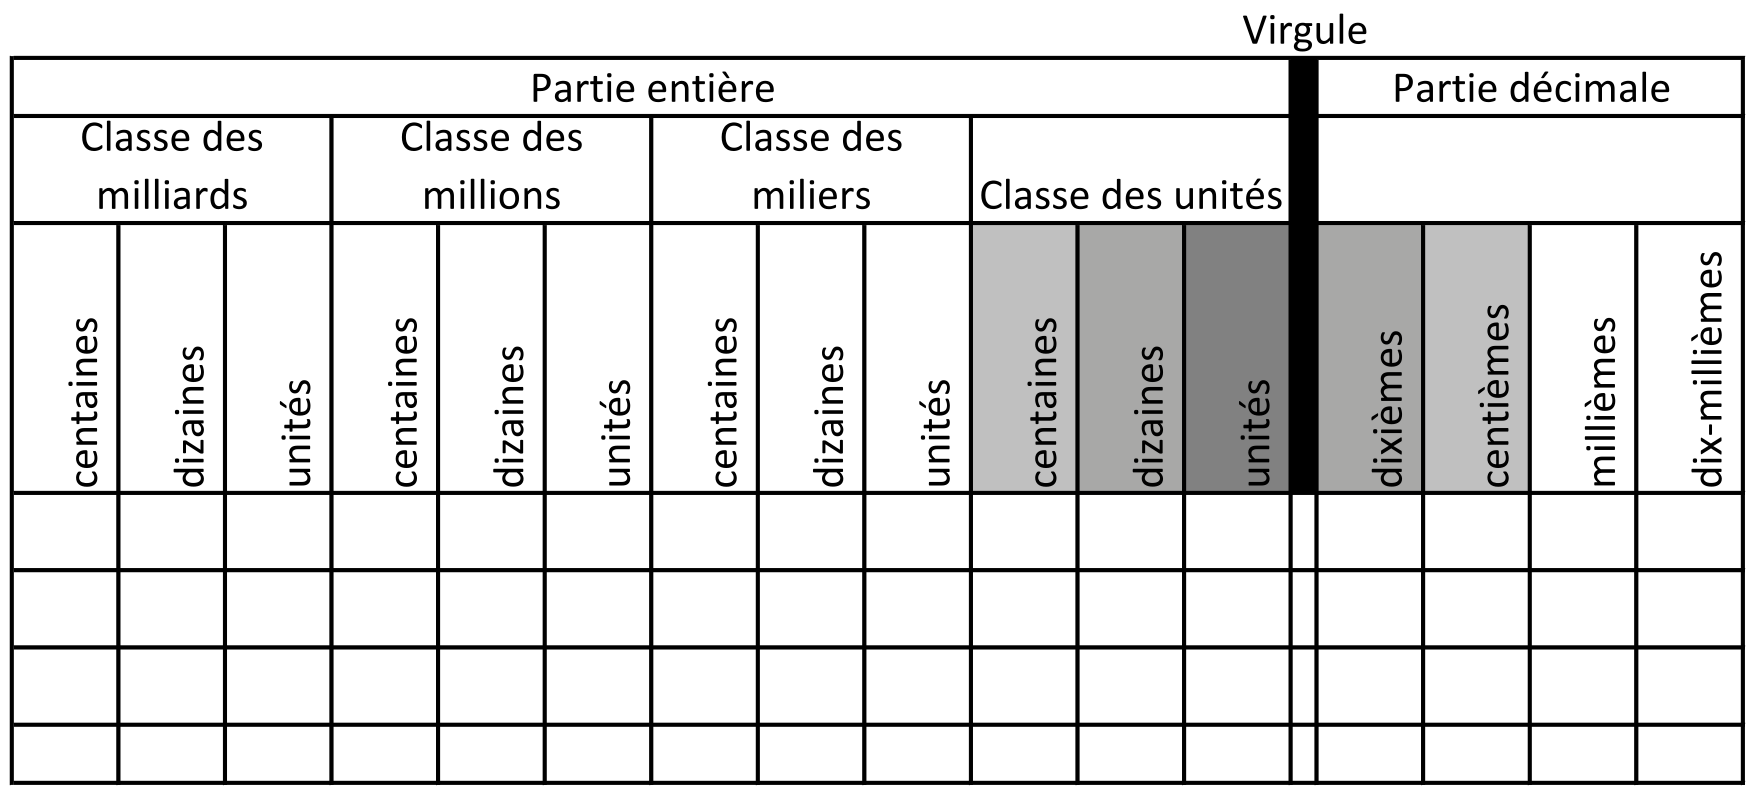
\includegraphics[scale=.25]{tab_rangs}\pause
	\end{center}

	\begin{exampleblock}{Exemples}
		\begin{itemize}
			\item Le nombre \num{2048} est un nombre entier composé de 4 chiffres différents.
			\item La partie entière de \num{5239.67}  est \num{5239} et sa partie décimale est 67.	
			
			\item Le nombre \num{124} peut aussi s'écrire \num{124.00}.
		\end{itemize}
	\end{exampleblock}
\end{frame}


\begin{frame}
	
	
	
	\begin{block}{Méthode}
		Pour \'ecrire un nombre en toutes lettres :\pause
		\begin{itemize}
			\item Tous les mots qui désignent un nombre sont invariables, sauf <<vingt>> et <<cent>>;\pause
			\item Les mots <<milliard>>, <<million>>, <<dixième>> ne désignent pas des nombres, ils prennent un <<s>> au pluriel;\pause
			\item 80 s'écrit <<quatre-vingts>> sauf s'il est suivi d'un autre nombre;\pause
			\item 100 s'écrit <<cents>> s'il est multiplié et non suivi d'un autre nombre, dans les autres cas il ne prend pas de <<s>>;\pause
			\item on écrit un trait d'union entre chaque mot d'un nombre.
		\end{itemize}
	\end{block}
\end{frame}
\end{document}